\documentclass{beamer}

\usepackage[utf8]{inputenc}
\usepackage{hyperref}
\usetheme{Madrid}
\usecolortheme{beaver}
\graphicspath{ {./img/} }

\title{Network flow}
%\subtitle{People often joke that in order to understand recursion, you must first understand recursion}
\author[Carocari, Fabris, Lotito]
{Giulia Carocari, Giacomo Fabris, Francesco Lotito}
\institute[UniTN]{Università degli Studi di Trento}
\date[May 2, 2019]
{ICPC Training @ UniTN\\ Day 7 - May 2, 2019}



\begin{document}

\frame{\titlepage}
\begin{frame} 
    \frametitle{Table of Contents}
    \tableofcontents
\end{frame}
\AtBeginSection[]{
    \begin{frame}
    \frametitle{Table of Contents}
    \tableofcontents[currentsection]
    \end{frame}
}
\AtBeginSubsection[]{
    \begin{frame}
    \frametitle{Table of Contents}
    \tableofcontents[currentsubsection]
    \end{frame}
}

\section{Solutions from last week's contest}

    \begin{frame}{A - Inflation}
        \begin{block}{Problem statement}
            Balloon capacity goes from $1$ to $n$, you are given the amount of helium in
            each of the $n$ helium canisters. Your goal is to assign gas canisters to balloons in 
            a way such that the least full balloon still contains the maximum possible fraction 
            of helium inside. If a ballon is filled beyond its capacity, it will explode.
        \end{block}
        \pause
        \setbeamercolor{block title}{use=structure,fg=white,bg=cyan!75!black}
        \begin{block}{Solution}
            \textbf{Greedy solution:}
            Sort canisters by the amount of gas. For each $i\in \{1..n\}$, store the minimum
            value of $gas[i]/i$, print \texttt{impossible} if you find such a value that is 
            greater than 1.
        \end{block}
    \end{frame}

    \begin{frame}{B - Frosting on the cake}
        \begin{block}{Problem statement}
            \begin{figure}[!htb]
                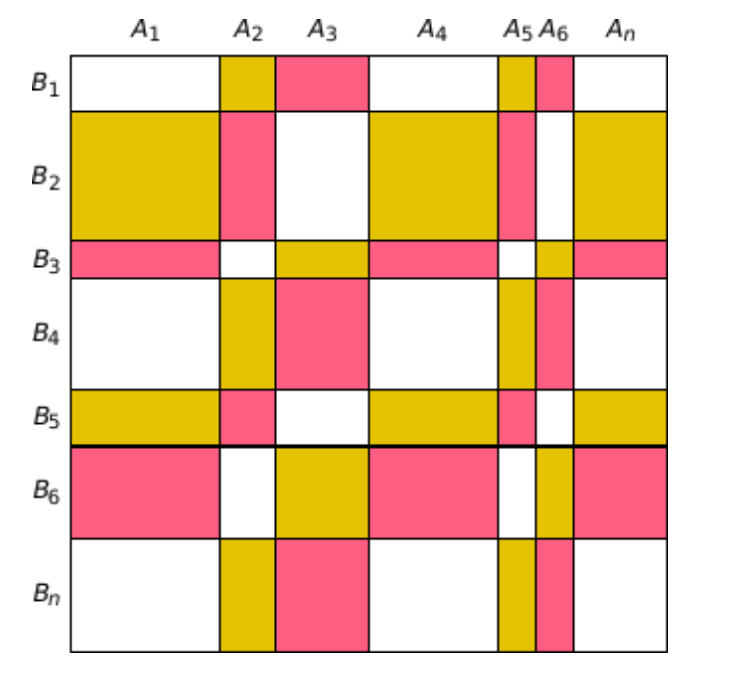
\includegraphics[width=50mm]{frosting}
            \end{figure}
            How big is the area covered by each color?\\
        \end{block}
        \alert{NOTE:} the dimensions of the grid are bounded by $10^5$, so the obvious
            $\mathcal{O}(nm)$ solution will get you a TLE.
    \end{frame}
    \begin{frame}{B - Frosting on the cake}
        \setbeamercolor{block title}{use=structure,fg=white,bg=cyan!75!black}
        \begin{block}{Solution}
            In fact, it is enough if you iterate over one dimension at a time. First compute
            sums $S_k$ of $A_i$, where $i\hspace{0.2em}mod\hspace{0.2em}3 = k$, for $k=0,1,2$.\\
            Then iterate over the $B_i$'s multiplying the $S_k$'s and summing to the correspondent
            counters of the color.
        \end{block}
        \alert{NOTE 1:} When implementing the solution pay attention to the fact that colors
        are numbered from 0 to 2, whereas the grid is indexed from 1 to $n$ and from 1 to $m$.\\
        \alert{NOTE 2:} Save yourself a lot of \texttt{C++} debugging using \texttt{long (long int)}
        numbers instead of regular 32-bit integers.  
    \end{frame}

    \begin{frame}{C - Cakey McCakeFace}
        \begin{block}{Problem statement}
            You want to find the cooking time of Cakey's cakes, so you place sensors at the entry
            and exit points of his oven. Unluckily, sometimes these sensors didn't trigger when a cake
            passed under them, other times they marked a timestamp without the need to.\\
            You want to find the cooking time that maximizes the association between plausible 
            entry and exit timestamps.
        \end{block}
        \pause
        \setbeamercolor{block title}{use=structure,fg=white,bg=cyan!75!black}
        \begin{block}{Solution}
            Compute all positive differences between input and output timestamps and use them as keys
            in a map. Use the value of a key as a counter to keep how many times you have encountered
            that cooking time. Print the smallest key with the maximum counter value.
        \end{block}
    \end{frame}

    \begin{frame}{D - Ingredients}
        \begin{block}{Problem statement}
            You are given a dependency graph on pizza recipes. Edges are marked by the cost to add an
            ingredient to another plate, nodes are labelled by the ``prestige'' of a dish.
            What is the maximum prestige you can obtain by staying within a given budget?
        \end{block}
        \pause
        \setbeamercolor{block title}{use=structure,fg=white,bg=cyan!75!black}
        \begin{block}{Solution}
            \textbf{Graphs + DP:}
            Compute a topological sort (to find dishes of cost 0), then 
            run a BFS to find the cost and prestige of each dish. Eventually apply 2-dimensional 
            dynamic programming to the computed costs/gains.
        \end{block}
    \end{frame}

    %%%%%%%%%%%%%%%%%%%%%%%%%%%%%%%%%%%%%%%%%%%%%%%%%%%%%%%%%%%%%%%%%%%%%%%%%%%%%%%%%%%%%%%%%%%%

    \section{Network flow}
    \subsection{MaxFlow Problem Definition}
    \begin{frame}{Analogies}
        Imagine a physical \textbf{network} of any kind: hydraulic pipes,
        computer networks, city maps, electric circuits...
        \begin{figure}[!htb]
            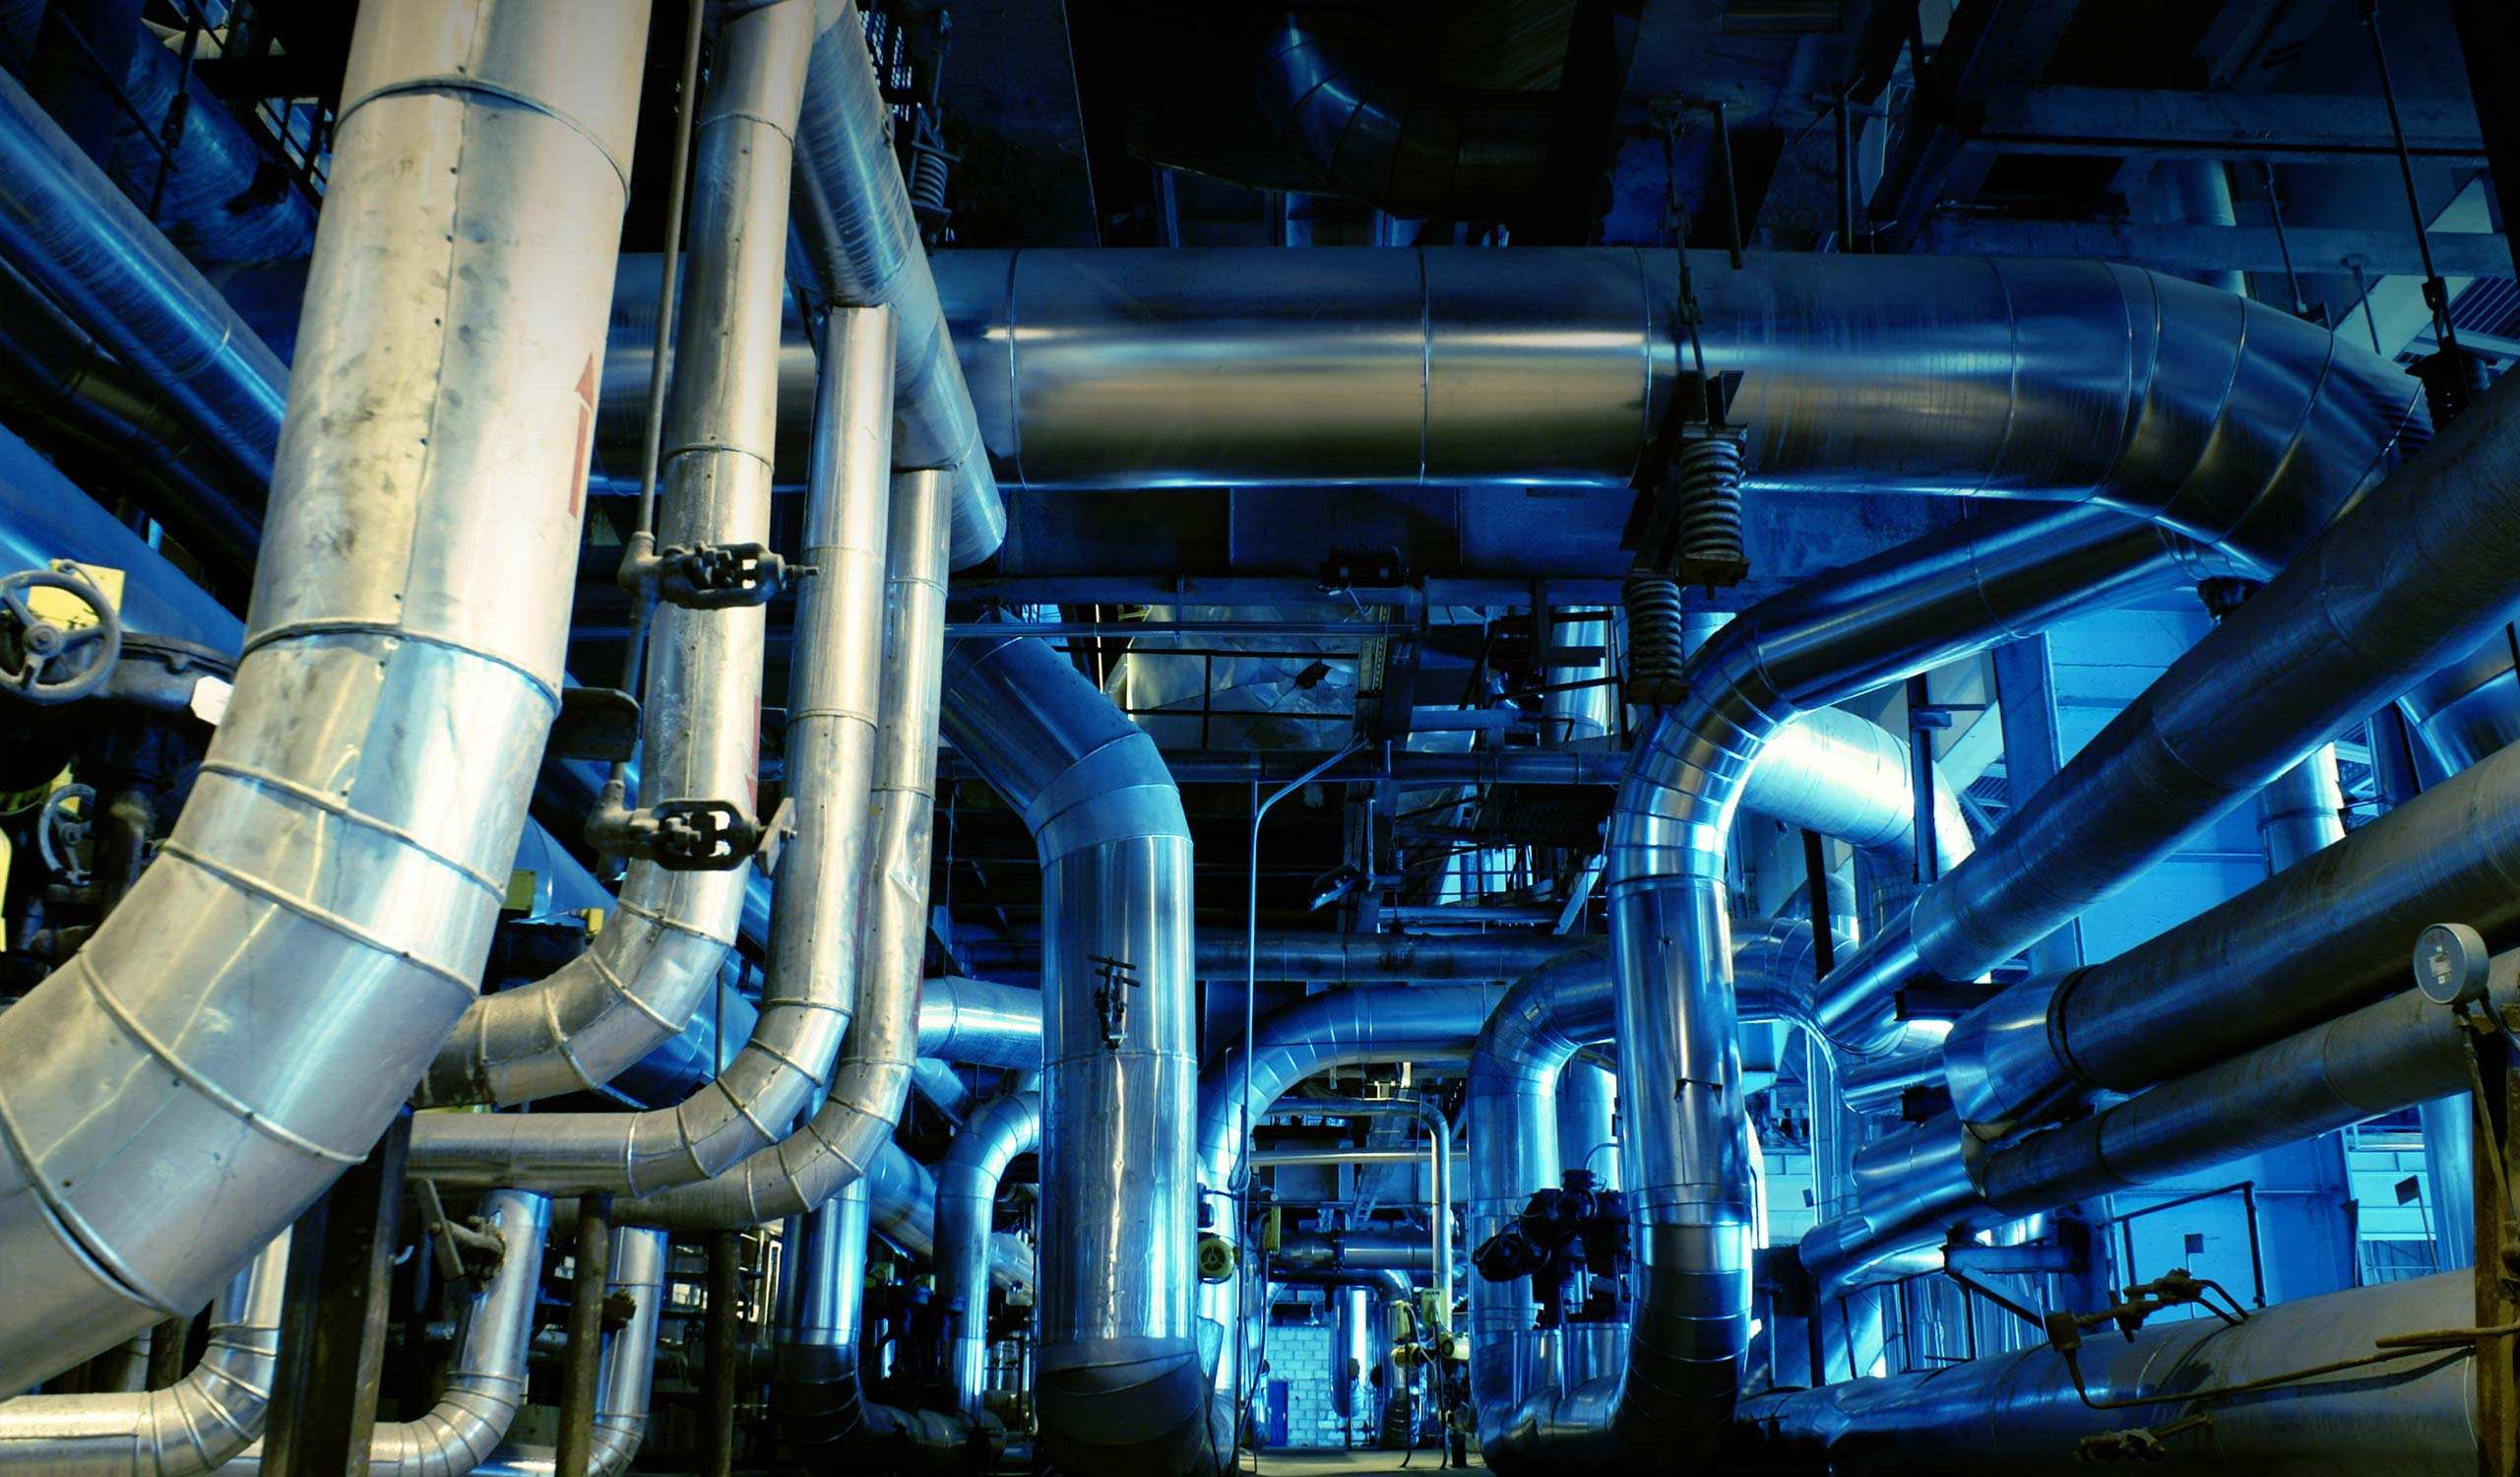
\includegraphics[width=50mm]{pipes}
        \end{figure}
        Each edge in this real-world graph (pipe, link, road, wire) has its own \textbf{capacity},
        i.e. a maximum amount of stuff (water, data, cars, electrons) that can travel
        along the connection in one time unit.
        What we want to compute in a \textbf{maximum flow problem} is the amount of ``stuff''
        we can have flowing in such networks between two special nodes called \textbf{source} and
        \textbf{sink}.
    \end{frame}

    \begin{frame}{Flow network}
        \begin{block}{Flow network}
            A graph where edges are labelled with positive capacities:
            $$c:V\times V\rightarrow \mathbb{R}^+$$
            such that if $(u,v) \notin E \Rightarrow c(u,v) = 0$.\\
            Two special nodes are identified, the source $s$ and the sink $t$.
        \end{block}
    \end{frame}

    \begin{frame}{Flow}
        \begin{block}{Flow}
            Formally it is a function:
            $$f:V\times V \rightarrow \mathbb{R}$$
            that associates flow values to each edge.
        \end{block}
        It must have the following properties:
        \begin{itemize}
            \item \textbf{Capacity bound:} $f(u,v)\leq c(u,v)$
            \item \textbf{Antisimmetry:} $f(u,v) = -f(v,u)$
            \item \textbf{Conservation of flow:} At every node (excluding source and sink)
                    the sum of entering and exiting flow must be 0.
        \end{itemize}
    \end{frame}

    \begin{frame}{Flow value}
        \begin{block}{Flow value}
            Once some flow has been injected into the network, we compute its value as:
            $$|f|=\sum_{u\in V} f(s,u)$$
        \end{block}
        This is the flow exiting from the source $s$.
        \begin{figure}[!htb]
            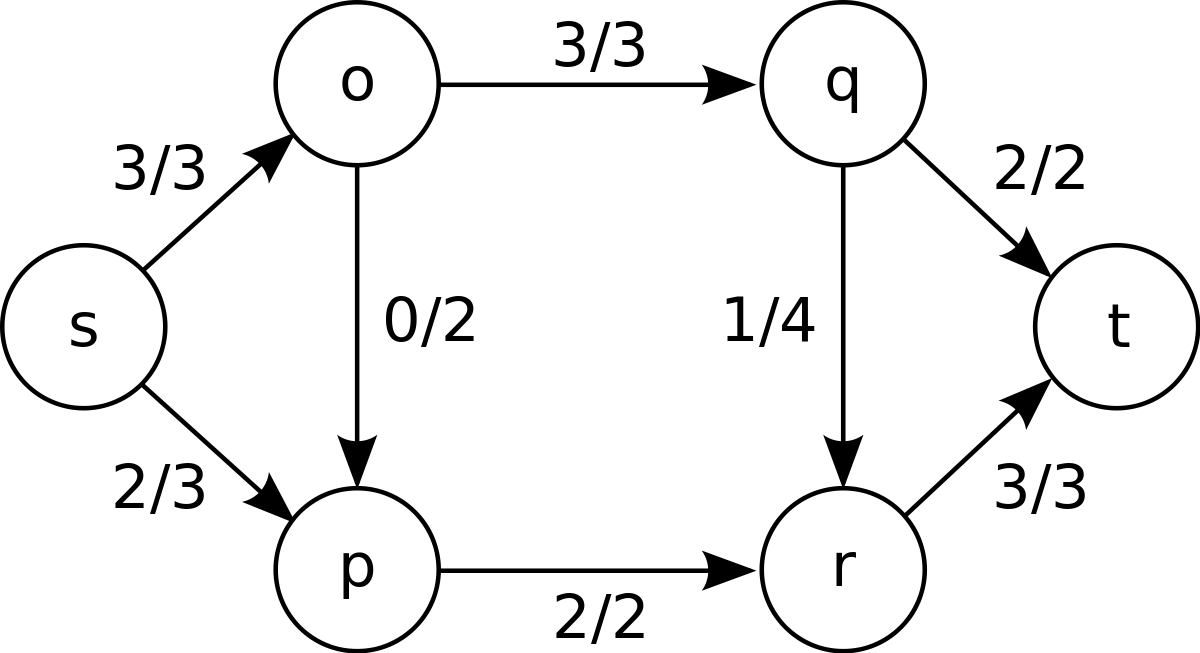
\includegraphics[width=60mm]{maxflow}
        \end{figure}
        \begin{flushright}
        \tiny{Source: \href{https://en.wikipedia.org/wiki/Maximum_flow_problem}{Wikipedia}}
        \end{flushright}
    \end{frame}

    \begin{frame}{Residual network}
        Once some flow $f$ has been injected into the network, we have a residual network, composed
        of the nodes of the original network and the edges labelled with the residual capacities
        $c_f(u,v)=c(u,v)-f(u,v)$
        \begin{block}{Residual network}
            The residual network is a structure $(V,E_f,c_f,s,t)$, where 
            $$(u,v)\in E_f \Leftrightarrow c_f(u,v) > 0$$
        \end{block}
        \alert{NOTE:} The original graph is a residual network where $f$ is the empty flow.
    \end{frame}

    \begin{frame}{Augmenting path}
        \begin{block}{Augmenting path}
            An augmenting path is a positive-flow path from the source to the sink in the
            current residual network.
        \end{block}
        \begin{alertblock}{Bottlenecks}
        The flow along an augmenting path $\mathcal{P}$ can be at most:
        $$min_{(u,v)\in P}\{c_f(u,v)\}$$
        We call this edge a \textbf{bottleneck}.
        \end{alertblock}
    \end{frame}

    \begin{frame}{Augmenting path}
        If we direct flow along the blue path in this residual network, its value must be at most
        2, in order not to violate the capacity bound.
        \begin{figure}[!htb]
            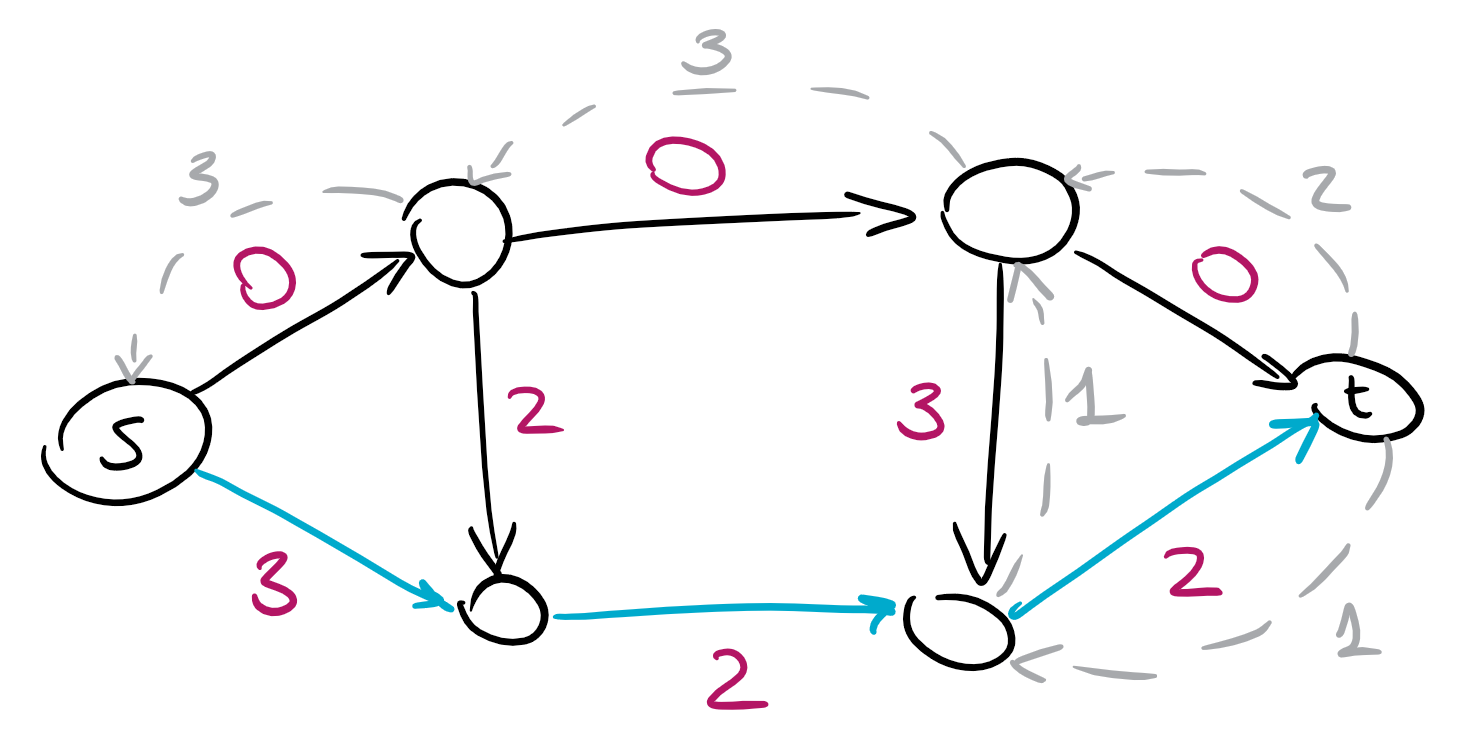
\includegraphics[width=110mm]{bottleneck}
        \end{figure}
    \end{frame}

    \begin{frame}{Why negative flow?}
        \begin{Large}
        We need the possibility to have flow into edges of capacity 0 in order to ``redirect''
        some flow along edges that were incorrectly added to the network by some augmenting paths.\\
        $$c(u,v) = 0 \land f(u,v) < 0 \Rightarrow c_f(u,v) > 0$$
        \end{Large}
    \end{frame}
    \subsection{Edmonds \& Karp's Algorithm}

    \begin{frame}{Ford \& Fulkerson}
        \begin{figure}
            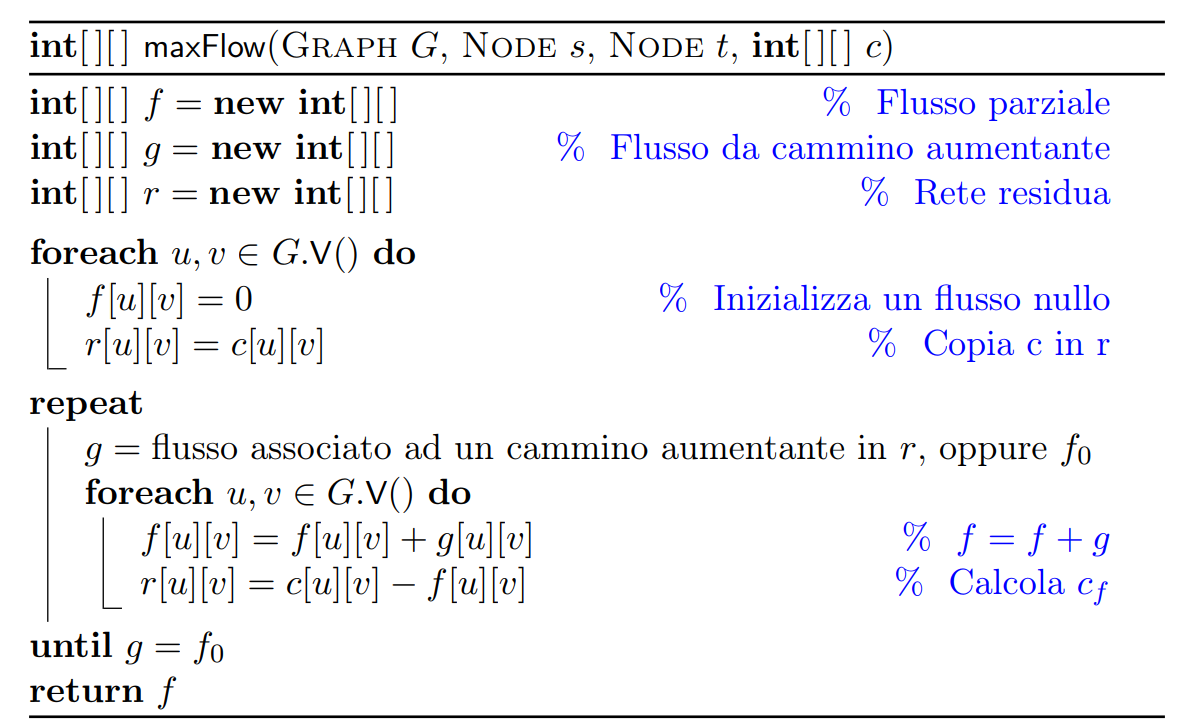
\includegraphics[width=120mm]{fordfulkerson}
        \end{figure}
    \end{frame}

    \begin{frame}{Ford \& Fulkerson}
        \begin{Large}
        The visit can be in any order you like, i.e. both BFS and DFS work. \vspace{24pt}\\
        \alert{Complexity:} $\mathcal{O}((V+E)|f^*|)$ (value of the maximum flow,
                which can be huge and/or hard to predict)
        \end{Large}
    \end{frame}

    \begin{frame}{Edmonds \& Karp}
        \begin{alertblock}{The smart way to search}
            Instead of searching for an augmenting path in any possible way (DFS or BFS)
            we can search for it using a BFS, thus diminishing the maximum number of such
            paths.
        \end{alertblock}
        \textbf{How does this work?} Every search for a path costs $\mathcal{O}(V+E)$ (BFS),
        but there are at most $\mathcal{O}(VE)$ of suitable shortest-paths.
        \\
        \textbf{Why does this hold?} Proof is left to the reader as exercise.
        \vspace{12pt}\\
        \alert{Complexity:} $\mathcal{O}(VE^2)$
    \end{frame}

    %%%%%%%%%%%%%%%%%%%%%%%%%%%%%%%%%%%%%%%%%%%%%%%%%%%%%%%%%%%%%%%%%%%%%%%%%%%%%%%%%%%%%%%%%%%%

    \subsection{Some other considerations about network flow problems}
    \begin{frame}{Min-cut}
        \begin{block}{Min-cut}
            Consider a graph $G=(V,E)$ and a function $c:E\rightarrow \mathbb{R}^+$.
            Partition the set $V$ into two sets $S$ and $T$, such that $s\in S$, $t\in T$ and:
            $$\sum_{u\in S, v\in T} c(u,v)$$
            is minimal.
        \end{block}
        \pause
        The value of the min-cut is exactly the value of the maximum flow $|f^*|$ 
        (\href{https://en.wikipedia.org/wiki/Max-flow_min-cut_theorem}{\underline{Max-flow min-cut theorem}}).
        \vspace{12pt}\\
        Informally, the edges that go from $S$ to $T$ are the bottlenecks of the max-flow problem,
        i.e. those edges with residual capacity 0 after running a Edmonds-Karp.
    \end{frame}

    \begin{frame}{Maximum cardinality bipartite matching}
        \begin{block}{Problem definition}
            Consider a bipartite graph $G=(U\cup V,E)$. Match each element in $U$ with
            exactly one node in $V$ with as many edges as possible (i.e. make as many
            matches as possible).
        \end{block}
        How?
        \begin{itemize}
            \item Edges in $E$ have capacity 1.
            \item Create a source connected to all elements in $U$ with capacity 1
            \item Connect all elements in $V$ with the sink (capacity 1).
        \end{itemize}
    \end{frame}

    \begin{frame}{Graph Modelling}
        \begin{block}{Multi-source \& multi-sink}
            Run Edmonds-Karp on a graph where two fresh nodes (a \textit{super-source} and
            a \textit{super-sink}) are connected by infinite-capacity edges to all sources and
            all sinks respectively.
        \end{block}

        \begin{block}{Vertex capacities}
            Each vertex $u$ is split into two components ($u_{in}, u_{out}$) connected by an
            edge such that:
            $$c(u_{in},u_{out}) = c(u)$$
        \end{block}
    \end{frame}
    \begin{frame}{Dinic's Algorithm (1970)}
        \begin{Large}
        Based on the concepts of \textbf{blocking flow} and \textbf{layered network}.
        \vspace{12pt}\\
        \alert{Complexity:} $\mathcal{O}(V^2E)$
        \vspace{12pt}\\
        See \href{https://cp-algorithms.com/graph/dinic.html}{\underline{this tutorial}}
        for the description and proofs of correctness and complexity.
        \end{Large}
    \end{frame}
\end{document}
